\documentclass[a4paper, 12pt]{report}

\def\languages{english, french}

%%%%%%%%%%%%%%%%%%% Libraries

\input{./include/libraries/bibliography.tex}
\input{./include/libraries/default.tex}
\input{./include/libraries/figures.tex}
\input{./include/libraries/mathematics.tex}
\input{./include/libraries/theorems.tex}
%%%%%%%%%% Packages

\usepackage[binary-units=true]{siunitx}

%%%%%%%%%% Features

%%%%% Settings

\ifx\decimalsign\undefined
\else
    \sisetup{output-decimal-marker = \decimalsign}
\fi


%%%%%%%%%%%%%%%%%%% Titlepage

\def\logopath{./resources/pdf/logo-uliege.pdf}
\def\toptitle{Université de Liège}
\title{Méthodes de Monte-Carlo par chaînes de Markov}
\def\subtitle{Éléments de processus stochastiques}
%\def\authorhead{}
\author{Maxime \textsc{Meurisse} (20161278)\\François \textsc{Rozet} (20161024)\\Valentin \textsc{Vermeylen} (20162864)\\}
%\def\rightauthorhead{}
%\def\rightauthor{}
\def\context{3\ieme{} année de Bachelier Ingénieur civil}
\date{Année académique 2018-2019\\\today}

%%%%%%%%%%%%%%%%%%% Bibliography

\addbibresource{resources/bib/ref.bib}

%%%%%%%%%%%%%%%%%%%

\def\MCMC{MCMC}

\makeatletter
\renewcommand{\@chapapp}{Partie}
\makeatother

%%%%%%%%%%%%%%%%%%%

\begin{document}
	\input{./include/titlepages/default.tex}
	\chapter{Chaînes de Markov et algorithme \MCMC}
	\section{Chaînes de Markov}
	\subsection{Matrice de transition, $\pi_0$ et diagramme d'états}
	Pour construire la matrice de transition $Q$, nous avons compté dans la séquence donnée le nombre de transitions d'un état $i$ à un état $j$, pour tout $i$ et $j$, et l'avons assigné à l'élément $q_{ij}$ de la matrice, conformément à la méthode du maximum de vraisemblance. En normant chaque ligne, nous obtenons
	\begin{equation}
	    Q =
	    \begin{pmatrix}
	        0 & 0 & \num{0.1605} & \num{0.8395} \\
	        \num{0.3226} & \num{0.5161} & \num{0.0968} & \num{0.0645} \\
	        \num{0.8644} & 0 & 0 & \num{0.1356} \\
	        \num{0.2564} & \num{0.1923} & \num{0.5513} & 0 \\
	    \end{pmatrix}
	\end{equation}
	que l'on peut représenter sous la forme d'un diagramme d'états (cf. figure \ref{fig:diagramme}).
	\begin{figure}[H]
	    \centering
	    \includegraphics[width=0.5\textwidth]{resources/tikz/diagram/diagram.pdf}
	    \noskipcaption{Diagramme d'états de la chaîne de Markov}
	    \label{fig:diagramme}
	\end{figure}
    Pour obtenir, ou plutôt avoir une chance d'obtenir, la séquence donnée, il faut initialiser la distribution de probabilités avec $1$ pour l'état initial de la séquence. Dans notre cas,
    \begin{equation}
	    \pi_0 =
	    \begin{pmatrix}
	        \num{1} & \num{0} & \num{0} & \num{0} \\
	    \end{pmatrix}
	\end{equation}
	\subsection{Calcul de grandeurs sur base de $Q$}
	Supposer que l'état initial est choisi au hasard revient à initialiser la distribution de probabilités initiale à un vecteur uniforme. À l'inverse, si l'état initial est toujours $3$, la probabilité de cet état est $1$. Nous avons donc respectivement
	\begin{align*}
	    \pi_0^a & =
	    \begin{pmatrix}
	        \num{0.25} & \num{0.25} & \num{0.25} & \num{0.25} \\
	    \end{pmatrix}
	    &
	    \pi_0^b & =
	    \begin{pmatrix}
	        \num{0} & \num{0} & \num{1} & \num{0} \\
	    \end{pmatrix}
    \end{align*}
    En multipliant itérativement ces distributions par la matrice de transition $Q$, nous obtenons leur évolution au cours des itérations $t$, données à la figure \ref{fig:evolutions}.
    \begin{figure}[H]
        \centering
        \begin{subfigure}{0.495\textwidth}
            \includegraphics[width=\textwidth]{resources/pdf/uniform.pdf}
            \caption{$\pi_0 = \pi_0^a$}
        \end{subfigure}
        \begin{subfigure}{0.495\textwidth}
            \includegraphics[width=\textwidth]{resources/pdf/determinist.pdf}
            \caption{$\pi_0 = \pi_0^b$}
        \end{subfigure}
        \noskipcaption{Évolution de la distribution de probabilités en fonction de celle initiale}
        \label{fig:evolutions}
    \end{figure}
    Nous observons que les deux distributions de probabilités tendent vers une même valeur. Pour $\num{50}$\footnote{Seules les $30$ premières itérations ont été représentées graphiquement pour ne pas rendre illisibles les quelques premières, plus pertinentes.} itérations, elles divergent à partir de la dixième décimale seulement et cette différence décroît rapidement lorsque le nombre d'itérations augmente.
    \begin{align*}
        \pi_{50}^a \simeq \pi_{50}^b \simeq
        \begin{pmatrix}
            \num{0.3253} & \num{0.1245} & \num{0.2369} & \num{0.3133} \\
        \end{pmatrix}
    \end{align*}
    Cela s'explique par le fait que les lignes de la $\num{50}$-ième puissance de $Q$ sont quasiment égales.
    \begin{align*}
        Q^{50} & =
        \begin{pmatrix}
	        \num{0.3253} & \num{0.1245} & \num{0.2369} & \num{0.3133} \\
	        \num{0.3253} & \num{0.1245} & \num{0.2369} & \num{0.3133} \\
	        \num{0.3253} & \num{0.1245} & \num{0.2369} & \num{0.3133} \\
	        \num{0.3253} & \num{0.1245} & \num{0.2369} & \num{0.3133} \\
	    \end{pmatrix}
    \end{align*}
    De ce fait, les produits de n'importe quelle distribution de probabilité avec cette dernière sont toujours identiques.\par
    Nous avons également calculé les puissances de la matrice de transition $Q$ pour des $t$ allant de $1$ à $50$. Les résultats pour quelques valeurs de $t$ sont repris ci-après.\par
    \begin{align*}
        Q^{5} & =
        \begin{pmatrix}
	        \num{0.3878} & \num{0.1373} & \num{0.2640} & \num{0.2110} \\
	        \num{0.3061} & \num{0.1362} & \num{0.2301} & \num{0.3276} \\
	        \num{0.2214} & \num{0.1204} & \num{0.2871} & \num{0.3711} \\
	        \num{0.3467} & \num{0.1097} & \num{0.1736} & \num{0.3700} \\
	    \end{pmatrix}
	    &
        Q^{10} & =
        \begin{pmatrix}
	        \num{0.3240} & \num{0.1268} & \num{0.2464} & \num{0.3028} \\
	        \num{0.3249} & \num{0.1242} & \num{0.2351} & \num{0.3158} \\
	        \num{0.3149} & \num{0.1221} & \num{0.2330} & \num{0.3300} \\
	        \num{0.3347} & \num{0.1240} & \num{0.2309} & \num{0.3104} \\
	    \end{pmatrix}
	    \\
        Q^{20} & =
        \begin{pmatrix}
	        \num{0.3251} & \num{0.1245} & \num{0.2370} & \num{0.3135} \\
	        \num{0.3253} & \num{0.1245} & \num{0.2369} & \num{0.3132} \\
	        \num{0.3255} & \num{0.1245} & \num{0.2368} & \num{0.3132} \\
	        \num{0.3253} & \num{0.1245} & \num{0.2371} & \num{0.3131} \\
	    \end{pmatrix}
	    &
        Q^{40} & =
        \begin{pmatrix}
	        \num{0.3253} & \num{0.1245} & \num{0.2369} & \num{0.3133} \\
	        \num{0.3253} & \num{0.1245} & \num{0.2369} & \num{0.3133} \\
	        \num{0.3253} & \num{0.1245} & \num{0.2369} & \num{0.3133} \\
	        \num{0.3253} & \num{0.1245} & \num{0.2369} & \num{0.3133} \\
	    \end{pmatrix}
    \end{align*}
    Nous constatons effectivement que les lignes de $Q$ tendent vers la distribution stationnaire $\pi_\infty$ pour des $t$ tendant vers l’infini.
    \subsection{Distribution stationnaire}
    Cette valeur vers laquelle nos distributions tendent irrémédiablement est appelée \emph{distribution stationnaire}.
    \begin{equation}
        \label{eq:distribution_stationnaire}
        \pi_{\infty} =
        \begin{pmatrix}
            \num{0.3253} & \num{0.1245} & \num{0.2369} & \num{0.3133} \\
        \end{pmatrix}
    \end{equation}
    En réalité, appliquer itérativement le produit de $Q$ à n'importe quelle distribution $\pi_0$ revient à appliquer la méthode de la puissance à $Q$. Pour rappel, cette méthode permet de trouver le vecteur propre de plus grande valeur propre en valeur absolue d'une matrice. \par
    Dès lors, $\pi_{\infty}$ est le vecteur propre à gauche de la matrice $Q$ associé à la valeur propre $1$ et cette dernière est la plus grande valeur propre en norme de $Q$.
    \subsection{Réalisations aléatoires}
    En démarrant d'un état choisi aléatoirement selon la distribution stationnaire \eqref{eq:distribution_stationnaire}, nous avons générés des réalisations aléatoires de longueur $T = 2^i$, pour $i$ allant de $1$ à $12$.\par
    Pour chaque réalisation aléatoire générée, nous avons calculé la fréquence d'apparition de chaque état. Les résultats obtenus sont présentés à la figure \ref{fig:stationnaire}.\par
    \begin{figure}[H]
        \centering
        \includegraphics[width=0.8\textwidth]{resources/pdf/frequency.pdf}
        \noskipcaption{Évolution des fréquences d'apparition des états pour réalisations aléatoires de tailles croissantes initialisées selon $\pi_\infty$.}
        \label{fig:stationnaire}
    \end{figure}
    Nous observons qu'à partir des réalisations de longueur $T = 256$\footnote{Cette longueur est fortement dépendante des tirages. Pour cette expérience, la longueur $2048$ semble plus raisonnable pour décréter les fréquences comme stabilisées.}, les fréquences d'apparition de chaque état sont assimilables à la distribution stationnaires $\pi_\infty$. Ce résultat s'affine et se confirme lorsque les valeurs de $T$ croissent.
    \subsection{Conclusion}
    Cette expérience nous a permis d'observer plusieurs choses.\par
    Premièrement, nous avons constaté que la chaîne de Markov modélisant la séquence \texttt{seq1.mat} donnée possédait une distribution stationnaire. Cela n'est pas étonnant puisqu'une chaîne de Markov à espace d'états fini (c'est le cas de notre chaîne car elle ne possède que 4 états distincts) possède au moins une distribution de probabilité stationnaire.\par
    De plus, en calculant des puissances de la matrice de transition $Q$, nous avons constaté que les lignes de celle-ci (pour des puissances tendant vers l'infini) correspondaient à la distribution stationnaire. Cela est le cas lorsque la chaîne est irréductible et apériodique. En examinant le diagramme d'état présenté à la figure \ref{fig:diagramme}, on remarque que la chaîne est bien irréductible (il est bien possible de passer d'un état $i$ à un état $j$ avec une probabilité non-nulle) et apériodique. \par
    % moyenne sur temps == moyenne sur espace
    Deuxièmement, nous avons observé qu'en générant des séquences aléatoires initialisées selon $\pi_\infty$, on obtenait des fréquences d'apparition des états assimilables à la distribution stationnaire. Cela s'explique par le fait que si une chaîne de Markov est initialisée selon une distribution stationnaire, ce qui est bien le cas ici, alors elle y restera pour tous les instants suivants.
	\section{Méthode \MCMC : Analyse théorique dans le cas fini}
	\subsection{Équations de balance}
    Considérons $\pi_1$, la distribution obtenue en appliquant la matrice $Q$ à la distribution $\pi_0$.
	\begin{align*}
	    \pi_1(i) & = \sum_j \pi_0(j) \, Q(j, i)
	\end{align*}
	Si $\pi_0$ satisfait aux équations de balance détaillée, à savoir
	\begin{align}
        \pi_0(i) \, Q(i, j) & = \pi_0(j) \, Q(j, i) \; & \forall i, j \in \cbk{1, \dots, N}
    \end{align}
    nous avons
	\begin{align*}
	    \pi_1(i) & = \sum_j \pi_0(i) \, Q(i, j) \\
	    & = \pi_0(i) \underbrace{\sum_j Q(i, j)}_{1} \\
	    & = \pi_0(i)
	\end{align*}
	Ainsi, $\pi_0 = \pi_1$ est une distribution stationnaire de la chaîne de Markov. \par
	Nous remarquons que cette démonstration est bidirectionnelle : une distribution stationnaire d'une chaîne de Markov respecte toujours les équations de balance détaillée. \par
	De plus, $\pi_0$ est l'unique distribution stationnaire si et seulement si la valeur propre $1$ de la matrice $Q$ n'est pas dégénérée. \par
	\subsection{Génération}
    Considérons les probabilités de transitions entre deux états $i$ et $j$ différents, la preuve du cas $i = j$ étant triviale.
	\begin{align*}
	    Q(i, j) & = q(j | i) \, \min \cbk{1, \frac{f(j)}{f(i)} \frac{q(i | j)}{q(j | i)}} \\
	    Q(j, i) & = q(i | j) \, \min \cbk{1, \frac{f(i)}{f(j)} \frac{q(j | i)}{q(i | j)}}
	\end{align*}
	Si $f(j) \, q(i | j)$ est plus grand que $f(i) \, q(j | i)$ :
	\begin{align*}
	    Q(i, j) & = q(j | i) \\
	    Q(j, i) & = q(j | i) \frac{f(i)}{f(j)}
	\end{align*}
	Sinon,
	\begin{align*}
	    Q(i, j) & = q(i | j) \frac{f(j)}{f(i)} \\
	    Q(j, i) & = q(i | j)
	\end{align*}
    Dans les deux cas, nous avons
	\begin{alignat*}{2}
	    && f(i) \, Q(i, j) & = f(j) \, Q(j, i) \\
	    \Leftrightarrow \quad && p_X(i) \, Q(i, j) & = p_X(j) \, Q(j, i)
	\end{alignat*}
	Dès lors, $p_X$ est une distribution stationnaire de la chaîne de Markov créée.\par 
	
	L'autre condition que la chaîne doit respecter afin que l'algorithme de Metropolis-Hastings fonctionne est l'ergodicité (apériodicité et irréductibilité), afin d'assurer une convergence unique, et donc une distribution $p_X$ unique (car la distribution stationnaire sera alors unique). Qui plus est, il faut également que $q$ couvre au moins le domaine de $p_X$ afin d'obtenir une distribution approximant correctement $p_X$. 
	\section{Application sur un exemple simple}
	\subsection{Distribution de proposition}
	Nous devons nous assurer que la matrice $Q(x, y)$ composée des lignes $q\rbk{y|x}$ est bien une matrice de transition. \par
	D'abord, on constate que la probabilité de chaque élément est soit $\frac{1}{2}$ soit $0$. Dès lors tous ses éléments sont compris entre $0$ et $1$ (\emph{premier axiome de Kolmogorov}). \par
	Ensuite, on observe que, pour chaque valeur de $x$, il existe deux valeurs de $y$ dont la probabilité associée est \num{0.5}. Les autres étant nulles, on a $\sum_y q\rbk{y|x} = 1$ (\emph{deuxième axiome de Kolmogorov}). \par
	
	Qui plus est, la distribution $q$ produit un processus ergodique. En effet,  tout état est accessible depuis tout autre état car 2 transitions sont non-nulles pour chaque état, et, les transitions non-nulles suivant les deux colonnes de part et d'autre de la diagonale principale, il est évident que chaque état permet d'atteindre tout autre état en un certain nombre de transitions. \cite{ergodicity} 
	\par
	Ainsi, $Q$ est bien une matrice de transition et l'algorithme permettra effectivement de générer des échantillons selon $p_X$.
	\subsection{Réalisation de la chaîne}
	\label{sec:etude_realisation}
	Les valeurs théoriques attendues de la moyenne et de la variance des réalisations $x$ sont celles de la distribution $p_X$, \cad{} d'une loi de Poisson. À savoir
	\begin{align*}
	    E\cbk{x} & = \lambda = 2 & V\cbk{x} & = \lambda = 2
	\end{align*}
    En réalité, la loi étant tronquée à $K = 10$, les moyenne et variance sont légèrement modifiées.
    \begin{align*}
	    E\cbk{x} & = \sum_{x = 0}^{K} x \, p_X(x) & V\cbk{x} & = \rbk{\sum_{x = 0}^{K} x^2 \, p_X(x)} - E\cbk{x}^2 \\
	    & = \num{1.999923619664117} & & = \num{1.999312571143103}
	\end{align*}
	En générant plusieurs réalisations de tailles croissantes nous observons que leurs moyenne et variance convergent vers les valeurs théoriques. Les résultats sont présentés à la table \ref{tab:moyenne_variance}.\par
	\begin{table}[H]
	    \centering
	    \begin{tabular}{|l|c|c|}
	        \hline
	        {\bf Taille de la réalisation} & {\bf Moyenne} & {\bf Variance} \\ \hline
	        \hline
	        \num{100} & \num{1.7200} & \num{1.3616} \\ \hline
	        \num{1000} & \num{2.1430} & \num{2.2266} \\ \hline
	        \num{10000} & \num{2.0418} & \num{1.9991} \\ \hline
	        \num{100000} & \num{2.0155} & \num{2.0189} \\ \hline
	        \num{1000000} & \num{2.0045} & \num{2.0076} \\ \hline
	    \end{tabular}
	    \noskipcaption{Moyenne et variance des valeurs générées pour plusieurs réalisations de tailles croissantes}
	    \label{tab:moyenne_variance}
	\end{table}
	\subsection{Distribution théorique}
	Nous avons tracé un histogramme permettant de comparer les fréquences d'apparition de chaque valeur dans une réalisation de taille \num{e4} et la distribution théorique. Celui-ci est présenté à la figure \ref{fig:histogram}. \par
	\begin{figure}[H]
	    \centering
	    \begin{subfigure}{0.48\textwidth}
	        \includegraphics[width=\textwidth]{resources/pdf/histogram_10000.pdf}
	        \caption{Réalisation de taille \num{e4}}
	    \end{subfigure}
	    \hspace{0.2em}
	    \begin{subfigure}{0.48\textwidth}
	        \includegraphics[width=\textwidth]{resources/pdf/histogram_1000000.pdf}
	        \caption{Réalisation de taille \num{e6}}
	    \end{subfigure}
	    \noskipcaption{Comparaison des fréquences $f$ d'apparition des entiers $\cbk{1, 2, \ldots, K}$ dans des réalisations et leur distribution théorique.}
	    \label{fig:histogram}
	\end{figure}
	Nous constatons que les distributions $f$ obtenues avec l'algorithme de Metropolis-Hastings sont proches de la distribution théorique $p_X$ et qu'augmenter la taille de la réalisation diminue l'erreur commise.
	\chapter{Problème d'optimisation combinatoire}
	\section{Description du problème}
	Le problème que nous avons choisi de résoudre est le problème du \emph{voyageur de commerce}. Ce problème consiste, étant donné un ensemble de $N$ points, à déterminer le plus court chemin partant d'un point, passant une et une seule fois par tous les autres points et revenant au point de départ.\par
	Notre algorithme sera testé sur trois ensembles de villes décrites par leurs coordonnées $(x, y)$.
    \begin{itemize}
        \item Les \num{38} villes du Djibouti, enregistrées dans le fichier \texttt{djibouti.txt};
        \item les \num{194} villes du Qatar, enregistrées dans le fichier \texttt{qatar.txt}; \cite{national_tsp}
    	\item les \num{2734} villes de Belgique, enregistrées dans le fichier \texttt{belgium.txt}.
    \end{itemize}
	
	
	Pour obtenir les distances entre les villes, nous utiliserons la distance euclidienne. Ainsi, la distance $d_{i,j}$ entre deux villes $i$ et $j$ sera
	\begin{equation}
	    d(i,j) = \sqrt{(x_i - x_j)^2 + (y_i - y_j)^2}
	\end{equation}
	Pour notre implémentation, l'espace $S$ des solutions contient l'ensemble des permutations des $N$ villes fournies. Un état/chemin $s$ de $S$ est donc défini comme une liste ordonnée de N couples $(x_i, y_i)$. \par
	Sur cet espace, nous cherchons à minimiser la fonction $f(s)$ définie comme la longueur totale du chemin $s$. En d'autres mots,
	\begin{equation}
	    f(s) = d(N,1) + \sum_{i = 1}^{N-1} d(i,i+1)
	\end{equation}
	\section{Cardinalité de l'espace des solutions}
	Pour des chemins de $N$ villes, il existe $\fact{N}$ permutations possibles. La cardinalité de notre espace est donc $\fact{N}$. \par
	Cependant, deux permutations cycliques d'un même chemin sont parfaitement équivalentes, de même qu'un chemin et son retournement. On peut alors montrer que le nombre de chemins non-équivalents est $\frac{1}{2} \fact{(N - 1)}$. \cite{wiki_tsp} \par
	Dans le cas de la Belgique, $N$ valant $\num{2734}$, $S$ possède de l'ordre de \ldots \num{e8207} chemins non-équivalents. Il n'est pas envisageable d'énumérer toutes ces solutions afin de trouver la plus courte. En effet, même en imaginant des ordinateurs capables de générer et calculer la longueur des permutations à une fréquence de \num{e20} permutations par seconde\footnote{Les meilleurs processeurs actuels peuvent effectuer de l'ordre de \num{e10} opérations basiques par seconde. Dès lors, des ordinateurs capables de \num{e20} opérations complexes par seconde ne sont pas près de voir le jour.}, il faudrait \num{e8180} années pour déterminer la solution de ce problème. À titre de comparaison, l'âge de notre univers est estimé à \num{14} milliard années.
	\section{Distribution de proposition $q$}
	Comme le proposait l'énoncé, nous avons opté pour une distribution $p_S$ du type
	\begin{equation*}
	    p_S(s) = Ce^{-\beta f(s)}
	\end{equation*}
	Ainsi, pour les états $s$ et $z$ remplaçant respectivement $x^{(t - 1)}$ et $y^{(t)}$, l'expression de $\alpha$ prend la forme
	\begin{align}
        \alpha & = \min \cbk{1, \frac{p_{S}(z)}{p_{S}(s)} \frac{q \rbk{s | z}}{ q \rbk{z | s}}} \nonumber \\
        & = \min \cbk{1, e^{-\beta f(z) + \beta f(s)} \frac{q \rbk{s | z}}{ q \rbk{z | s}}} \nonumber \\
        & = \min \cbk{1, e^{-\beta \Delta(s, z)} \frac{q \rbk{s | z}}{ q \rbk{z | s}}}
    \end{align}
    où $\Delta(s, z) = f(z) - f(s)$ est la variation de la fonction $f$ à minimiser en passant de l'état $s$ à l'état $z$. \par
    Il reste donc à choisir $q$ pour permettre à l'algorithme de converger au plus vite.
	\subsection{Première idée}
    Pouvoir passer, aléatoirement ou non, de n'importe quel état à n'importe quel autre à chaque itération de l'algorithme est assez peu judicieux. En effet, cela nécessite de générer entièrement le nouvel état et de calculer sa longueur à chaque itération ce qui peut-être très coûteux numériquement. \par
    À la place, notre première idée était de restreindre les états accessibles à partir d'un chemin $s$ aux chemins identiques à $s$ mais où deux points \emph{consécutifs} avaient été permutés. Cet ensemble d'états accessibles $Z_s$ comporte donc toujours $N$ états. \par
    L'avantage principal de cette méthode est que le calcul de $\Delta$ est très réduit.
    Pour orienter le choix parmi ces états, nous avons décidé de favoriser les états $z$ qui diminuent la longueur du chemin par rapport à $s$, \cad{} les états $z$ tels que $\Delta(s, z)$ est négatif. \par
    Nous avons alors pensé à une exponentielle négative, et notre distribution de proposition $q$ fut définie comme
    \begin{equation}
        q\rbk{z | s} =
        \begin{cases}
            D_s \, e^{\gamma \Delta(s, z)} & \forall z \in Z_s \\
            0 & \forall z \in S \setminus Z_s
        \end{cases}
    \end{equation}
    où $D_s$ est une constante de normalisation telle que $\sum_{z \in S} q\rbk{z | s} = 1$ et $\gamma$ un paramètre arbitraire. \par
    En implémentant cette distribution de probabilité, nous avons remarqué que si l'ensemble des états accessibles était relativement restreint, il n'en était pas pour autant facile d'y piocher. En effet, pour effectuer cette action, il fallait au préalable déterminer les $N$ valeurs non triviales de $q(z|s)$.
    \subsection{Deuxième idée}
    Avec la distribution décrite à la section précédente, $\alpha$ devient
    \begin{align*}
        \alpha & = \min \cbk{1, e^{-\beta \Delta(s, z)} \frac{D_z}{D_s} e^{-\gamma \Delta(s, z)}} \\
        & = \min \cbk{1, \frac{D_z}{D_s} e^{-(\beta + \gamma) \Delta(s, z)}}
    \end{align*}
    En supposant $N$ très grand, on peut affirmer que les coefficients $D_s$ d'un chemin $s$ et $D_z$ d'un de ses chemins accessibles $z$ sont très proches. Si proche que leur quotient est très certainement négligeable vis à vis d'une exponentielle. En faisant cette approximation,
    \begin{align*}
        \alpha & = \min \cbk{1, e^{-(\beta + \gamma) \Delta(s, z)}}
    \end{align*}
    Nous remarquons que cet $\alpha$ est en réalité parfaitement équivalent à celui d'un algorithme où nous aurions choisi $\beta' = \beta + \gamma$ et une distribution de probabilité uniforme sur $Z_s$.
    Ainsi,
    \begin{equation}
        q\rbk{z | s} =
        \begin{cases}
            \frac{1}{N} & \forall z \in Z_s \\
            0 & \forall z \in S \setminus Z_s
        \end{cases}
    \end{equation}
    et
    \begin{equation} \label{eq:alpha}
        \alpha = \min \cbk{1, e^{-\beta \, \Delta(s, z)}}
    \end{equation}
    \subsection{Troisième idée} \label{sec:troisieme_idee}
    L'idée précédente a l'avantage d'être très simple à implémenter et converge rapidement vers une solution acceptable. Cependant, cette solution n'est que très rarement optimale. En effet, lorsque les $N$ chemins de $Z_s$ sont plus longs que $s$, \cad{} lorsqu'il atteint un minimum local, l'algorithme stagne. \par
    Afin de supprimer, ou plutôt amoindrir, ce problème, il faut augmenter le nombre d'états accessibles à partir de $s$. Nous avons donc décidé d'élargir l'ensemble $Z_s$ aux chemins identiques à $s$ mais où deux points \emph{quelconques} ont été permutés. La taille de $Z_s$ est donc égale au nombre de manières de choisir, sans ordre, deux éléments parmi un ensemble de $N$ éléments, \cad{} $\frac{1}{2}N(N-1)$. \par
    Finalement,
    \begin{equation} \label{eq:q}
        q\rbk{z | s} =
        \begin{cases}
            \frac{2}{N(N-1)} & \forall z \in Z_s \\
            0 & \forall z \in S \setminus Z_s
        \end{cases}
    \end{equation}
    Bien que cela soit difficile à justifier mathématiquement, nous pouvons affirmer que tout état est accessible à partir de n'importe quel autre avec cette distribution de probabilité, de par son design (on peut, à partir d'un chemin quelconque, permuter des éléments deux à deux de manière à atteindre n'importe quel autre chemin). La chaîne de Markov générée sera donc ergodique, comme le requiert l'algorithme de Metropolis-Hastings.
	\section{Implémentation et optimisation}
	Une itération de notre algorithme de Metropolis-Hastings se décompose en quatre parties :
	\begin{enumerate}
	    \item Choisir $z$ selon l'équation \eqref{eq:q}.
	    \item Déterminer $\Delta(s, z)$, \cad{} soustraire $f(s)$ à $f(z)$.
        \item Calculer $\alpha$ sur base de l'équation \eqref{eq:alpha}.
        \item Décider si $s$ est remplacé par $z$, avec une probabilité $\alpha$ de le faire.
	\end{enumerate}
	Les $M$ itérations constituant la majorité du temps d'exécution de l'algorithme, nous avons réalisé plusieurs optimisations dans l'implémentation \texttt{MATLAB} de ces quatre parties, afin de réduire au maximum les temps de calcul.
	\subsection{Choix du prochain chemin}
	Comme nous l'avons expliqué à la section \ref{sec:troisieme_idee}, le choix du prochain chemin se fait uniformément parmi les $\frac{1}{2} N (N - 1)$ éléments de l'ensemble $Z_s$. Ces derniers peuvent être décrits comme les chemins $z_{ij}$ ($i > j$) identiques à $s$ mais où le point $i$ a été permuté avec le point $j$. Dès lors, choisir un élément parmi $Z_s$ revient à tirer aléatoirement 2 nombres entre $1$ et $N$. \par
	Dans notre implémentation, ce tirage aléatoire se fait à l'aide de la fonction \texttt{randi}. Cependant, la distribution de probabilité étant uniforme, les tirages ne sont pas influencés par le chemin courant à l'itération. Dès lors, il est possible de les réaliser en amont de la boucle en un seul appel de \texttt{randi} et ainsi gagner un temps précieux. \par
	Cependant, cette méthode demande de stocker en mémoire les $M$ couples $(i, j)$ tirés. Le nombre d'itérations pouvant prendre des valeurs très élevées (jusqu'à \num{e10}) dans nos simulations, nous avons plutôt choisi d'appeler la fonction \texttt{randi} toutes les \num{e6} itérations.
	\subsection{Variation de la fonction $f$}
	Pour déterminer $\Delta(s, z_{ij})$, la première idée venant à l'esprit est de simplement calculer $f(s)$ et $f(z_{ij})$ pour en faire la différence. Cela signifie sommer les $N$ distances entre les points de $z_{ij}$, $f(s)$ ayant déjà été déterminé à l'itération précédente. Or, en y réfléchissant, nous avons remarqué que, mis à part huit (ou quatre selon le cas) d'entre elles, ces distances sont communes à $s$ et $z_{ij}$. \par
	Ainsi, pour déterminer $\Delta(s, z_{ij})$, on peut ne considérer que celles qui varient. On a,
    \begin{align*}
        \Delta(s, z_{ij}) & = f(z_{ij}) - f(s) \\
        & =
        \begin{cases}
            d(i-1,j) + d(i,j+1) - d(i-1,i) - d(j,j+1) & \forall \, i = j - 1 \\[0.5em]
            d(i-1,j) + d(j,i+1) + d(j-1,i) + d(i,j+1) & \forall \, i \neq j - 1 \text{ et} \\
            - d(i-1,i) - d(i,i+1) - d(j-1,j) - d(j,j+1) & i \neq 1 \text{ et } j \neq N \\[0.5em]
            d(N,j) + d(j,i+1) + d(j-1,i) + d(i,j+1) & \forall \, i = 1 \text{ et } j \neq N \\
            - d(N,i) - d(i,i+1) - d(j-1,j) - d(j,j+1) & \\[0.5em]
            d(i-1,j) + d(j,i+1) + d(j-1,i) + d(i,1) & \forall \, i \neq 1 \text{ et } j = N \\
            - d(i-1,i) - d(i,i+1) - d(j-1,j) - d(j,1) & \\[0.5em]
            d(N,2) + d(N-1,1) - d(1,2) - d(N-1,N) & \forall \, i = 1 \text{ et } j = N \\
        \end{cases}
    \end{align*}
	En moyenne, le calcul de $\Delta(s, z_{ij})$ demande donc de connaître $K$ distances\footnotemark{} entre des points du problème. Si $M$ est grand, recalculer ces distances à chaque itération peut devenir très coûteux numériquement. \par
	\footnotetext{$$ K = \frac{4 N + 8 \rbk{\frac{1}{2} N (N - 1) - N}}{\frac{1}{2} N (N - 1)} = \frac{8(N - 2)}{(N - 1)} \xrightarrow{\; N \rightarrow \infty \;} 8 $$}
    Pour éviter ces calculs à l'exécution et augmenter drastiquement la vitesse de notre implémentation, nous avons choisi de les réaliser en amont en calculant toutes les distances $d(i,j)$ et en les stockant dans une matrice $D$ telle que $D_{ij} = d(i,j)$. Cette dernière étant symétrique, nous n'avons calculé que $\frac{1}{2} N^2$ éléments. \par
    La matrice $D$ ne différant pas de simulation en simulation, nous avons décidé de la sauvegarder physiquement dans un fichier \texttt{.mat} au moment de sa première initialisation.
    \begin{table}[H]
        \centering
        \begin{tabular}{|c|c|c|}
            \hline
            Instance & Temps moyen de calcul $\sbk{\si{\second}}$ & Espace en mémoire \\ \hline\hline
            Djibouti & \num{0.003} & \SI{9.8}{\kilo\byte} \\ \hline
            Qatar & \num{0.038}  & \SI{278}{\kilo\byte} \\ \hline
            Belgique & \num{5.107} & \SI{54}{\mega\byte} \\ \hline
        \end{tabular}
        \noskipcaption{Calcul et sauvegarde de la matrice $D$ sur les serveurs de l'institut Montefiore.}
    \end{table}
    Si le temps de calcul est loin d'être déraisonnable, l'espace utilisé en mémoire est clairement une faiblesse de cette méthode.
    \subsection{Détermination de $\alpha$}
    En observant l'équation $\eqref{eq:alpha}$, nous avons remarqué que si $\Delta$ est négatif, l'exponentielle est supérieure à $1$ et $\alpha$ vaut nécessairement $1$. De la même manière, lorsque $\Delta$ est positif, l'exponentielle est inférieure à $1$ et $\alpha$ vaut obligatoirement cette valeur. \par
    Nous avons donc économisé l'utilisation de la fonction \texttt{min} et le calcul de l'exponentielle lorsque $\Delta$ est négatif.
    \subsection{Remplacement}
    Lorsque $\alpha$ vaut $1$, le chemin $s$ est automatiquement remplacé par le chemin $z_{ij}$, sans générer de nombre aléatoire. \par
    Aussi, pour ne pas réaffecter un vecteur complet, seuls les éléments $i$ et $j$ sont échangés dans le cas d'un remplacement.
    \subsection{Algorithme du plus proche voisin}\label{sec:NNA}
    Au lieu de commencer avec un chemin quelconque, nous avons utilisé un algorithme déterministe afin d'obtenir un chemin initial plus prometteur que le chemin aléatoire. Cet algorithme est celui du plus proche voisin \cite{wiki_nna} et fut un des premiers algorithmes utilisés pour obtenir des solutions acceptables au problème du voyageur de commerce. Son principe est très simple : \par 
    Le premier point du chemin est choisi arbitrairement puis les points suivants sont choisis de telle façon que la distance entre le point $i$ et le point $i + 1$ est la plus petite parmi les distances entre le point $i$ et les points $j > i$. \par
    Pour notre implémentation, nous avons décidé d'appliquer l'algorithme avec chacun des points de l'ensemble comme point initial du chemin pour choisir par après le plus court des chemins générés.
    \begin{table}[H]
        \centering
        \begin{tabular}{|c|c|c|}
            \hline
            Instance & Temps moyen de calcul $\sbk{\si{\second}}$ & Longueur $\sbk{\si{\kilo\meter}}$ \\ \hline\hline
            Djibouti & \num{0.009} & \num{6770.1} \\ \hline
            Qatar & \num{0.155} & \num{11330.4} \\ \hline
            Belgique & \num{198.4} & \num{8822.3} \\ \hline
        \end{tabular}
        \noskipcaption{Application de l'algorithme du plus proche voisin sur les serveurs de l'institut Montefiore.}
        \label{tab:nearest_neighbor_algorithm}
    \end{table}
    Comme le montre la Table \ref{tab:nearest_neighbor_algorithm}, le temps de calcul de ces chemins grandit très vite avec le nombre de points de l'instance du problème. De fait, une seule application de l'algorithme étant $\mathcal{O}(N^2)$, les $N$ applications que nous en faisons sont $\mathcal{O}(N^3)$ ce qui est généralement très mauvais\footnote{En réalité, nous aurions pu nous satisfaire d'une seule application de l'algorithme du plus proche voisin, mais nous avons préféré privilégier la qualité du chemin initial à quelques minutes de calcul.}. \par
    Néanmoins, comme la matrice $D$, ce chemin ne varie pas de simulation en simulation. Il n'est donc calculé qu'une seule fois\footnote{Le chemin initial ainsi que $D$ sont calculés à la première exécution de l'algorithme pour une instance donnée. Nous conseillons de lancer une simulation factice, avec peu d'itérations, avant d'effectuer les tests réels.} puis sauvegardé dans le même fichier \texttt{.mat} que $D$.
    \subsection{Temps de calcul}
    Toutes ces optimisations ont permis de gagner un temps considérable lors de l'exécution des simulations. De plus, grâce à la bonne gestion des matrices de grande taille de \texttt{Matlab}, le temps par itération ne dépend que faiblement de la taille de l'instance du problème.
    \begin{table}[H]
    	\centering
    	\begin{tabular}{|c|c|c|c|c|}
    		\hline
    		\multirow{2}{*}{Instance} & \multicolumn{4}{c|}{$M$} \\ \cline{2-5}
    		 & \num{e5} & \num{e6} & \num{e7} & \num{e8} \\ \hline
    		\hline
    		Djibouti & \SI{0.0215}{\second} & \SI{0.1703}{\second} & \SI{1.6925}{\second} & \SI{16.6340}{\second} \\ \hline
    		Qatar & \SI{0.0203}{\second} & \SI{0.1695}{\second} & \SI{1.7036}{\second} & \SI{16.8380}{\second} \\ \hline
    		Belgique & \SI{0.0289}{\second} & \SI{0.3209}{\second} & \SI{3.1833}{\second} & \SI{31.3650}{\second} \\ \hline
    	\end{tabular}
    	\noskipcaption{Temps d'exécution moyens de simulations réalisées sur les serveurs de l'institut Montefiore.}
    \end{table}
    \newpage
	\section{Analyse de la vitesse de convergence}
    Pour étudier la convergence de notre algorithme en fonction du paramètre $\beta$, nous nous baserons sur les solutions optimales $s^*$ des trois instances étudiées.
    \begin{table}[H]
    	\centering
    	\begin{tabular}{|c|c|}
    		\hline
    		Instance & Longueur de $s^*$ $\sbk{\si{\kilo\meter}}$ \\ \hline
    		\hline
    		Djibouti & \num{6659} \\ \hline
    		Qatar & \num{9352} \\ \hline
    		Belgique & \num{7212} \\ \hline
    	\end{tabular}
    	\noskipcaption{Longueurs des solutions optimales des instances du problème.}
    	\label{tab:optimal_solutions}
    \end{table}
    Ces solutions ont été déterminées à l'aide du solver \href{https://neos-server.org/neos/solvers/co:concorde/TSP.html}{\texttt{Concorde}} mis à disposition sur le \href{https://neos-server.org/neos/}{\texttt{NEOS Server}}.
    \subsection{Convergence}
    Pour analyser la vitesse de convergence, il faut au préalable choisir une manière de quantifier la convergence. Pour ce faire, nous avons défini la qualité d'une solution comme le rapport de sa longueur à celle de la solution optimale $s^*$. \par
    Ainsi, si la qualité tend vers $1$, c'est que l'algorithme converge. La convergence d'une simulation sera donc définie comme la différence de qualité entre la solution initiale $s_{ini}$ et la solution minimale $s_{min}$ (la meilleure solution trouvée au cours des itérations) :
    \begin{equation}
        \frac{f(s_{ini}) - f(s_{min})}{f(s^*)}
    \end{equation}
    Logiquement, la vitesse de convergence d'une simulation correspondra à sa convergence rapportée sur son nombre d'itérations. \par
    Cependant, à cause du hasard inhérent à l'algorithme de Metropolis-Hastings, la solution minimale et sa longueur varient parfois significativement entre deux simulations de paramètres identiques. Dès lors, la vitesse de convergence de l'algorithme sera analysée à partir d'une moyenne des longueurs des solutions minimales de plusieurs simulations.
    \subsection{Définition du paramètre \emph{beta}}
    Dans notre algorithme, le paramètre \emph{beta} est défini comme
    \begin{equation*}
        \beta_{rel} = \beta\rbk{\frac{N}{f(s_{ini})}}
    \end{equation*}
    Le facteur multiplicatif permet de rendre \emph{beta} relatif à la distance moyenne entre les points de l'instance étudiée. Ainsi, l'argument de l'exponentielle (cf. Eq. \eqref{eq:alpha}) est adimensionnel et le choix de \emph{beta} devient indépendant de l'instance étudiée. \par
    Par la suite, il s'agit bien de la valeur $\beta$ et non $\beta_{rel}$ que nous ferons varier.
    \subsection{Initialisation aléatoire}
    Pour cette première analyse, nous déterminons le chemin initial de chaque simulation de manière aléatoire. Afin d'avoir une idée de la longueur des chemins initiaux, nous avons noté leur ordre de grandeur et qualité approximatives, à la Table \ref{tab:random_initialization}.
    \begin{table}[H]
    	\centering
    	\begin{tabular}{|c|c|c|}
    		\hline
    		Instance & Longueur approximative de $s_{ini}$ $\sbk{\si{\kilo\meter}}$ & Qualité de $s_{ini}$ \\ \hline
    		\hline
    		Djibouti & \num{27000} & \num{4.0}\\ \hline
    		Qatar & \num{90000} & \num{9.3}\\ \hline
    		Belgique & \num{240000} & \num{33.6}\\ \hline
    	\end{tabular}
    	\caption{Longueurs et qualités approximatives des chemins initiaux des instances du problème, initialisées de manière aléatoire.}
    	\label{tab:random_initialization}
    \end{table}
    \subsubsection{Première évaluation}
    Afin d'évaluer une première fois le comportement de l'algorithme, nous avons décidé de travailler avec 7 valeurs fixes de $\beta$, d'ordre de grandeur différent : \num{0.01}, \num{0.1}, \num{1}, \num{10}, \num{100}, \num{1000} et \num{10000}.\par
    Pour chacune de ces valeurs, nous avons lancé plusieurs fois l'algorithme avec \num{e7} itérations et en avons fait des moyennes, présentées à la table \ref{tab:beta_for_random}.\par
    \begin{table}[H]
    	\centering
    	\begin{tabular}{|c|c|c|c|c|c|c|c|}
    	\hline
    		\multirow{2}{*}{Instance} & \multicolumn{7}{c|}{$\beta$} \\ \cline{2-8}
    		 & \num{0.01} & \num{0.1} & \num{1} & \num{10} & \num{100} & \num{1000} & \num{10000}\\ \hline
    		\hline
    		Djibouti & \num{17905} & \num{17456} & \num{14122} & \num{6659} & \num{8199} & \num{10783} & \num{10421}\\ \hline
    		Qatar & \num{76631} & \num{74664} & \num{56676} & \num{15143} & \num{15234} & \num{19155} & \num{19528}\\ \hline
    		Belgique & \num{233710} & \num{228547} & \num{56796} & \num{45197} & \num{31759} & \num{34562} & \num{35526}\\ \hline
    	\end{tabular}
    	\noskipcaption{Longueurs moyennes des chemins calculés des instances du problème, pour différentes valeurs de $\beta$ et une initialisation aléatoire.}
    	\label{tab:beta_for_random}
    \end{table}
    Nous constatons que, pour les différentes instances du problème, chaque valeur de $\beta$ semble mener à un chemin meilleur (voir bien meilleur) que celui initial.
    \subsubsection{Deuxième évaluation}
    Nous pourrions garder toutes les valeurs de $\beta$ pour effectuer des tests, mais, au vu des résultats précédents et afin d'alléger le nombre de résultats présentés, nous conserverons uniquement $\beta = \num{0.1}$ et $\beta = \num{10}$ pour la suite de l'analyse.\par
    Pour évaluer la vitesse de convergence de ces valeurs de $\beta$, nous avons relancé l'algorithme avec des nombres d'itérations croissants. Les qualités des solutions obtenues sont présentées à la table \ref{tab:quality_for_random}.\par
    \begin{table}[H]
    	\centering
    	\begin{tabular}{|l|c|c|c|c|c|c|}
    		\hline
    		$\beta$ & \multicolumn{3}{c|}{\num{0.1}} & \multicolumn{3}{c|}{\num{10}} \\ \hline
    		Nombre d'itérations & \num{e5} & \num{e6} & \num{e7} & \num{e5} & \num{e6} & \num{e7}\\ \hline
    		\hline
    		Djibouti & \num{2.8649} & \num{2.8482} & \num{2.6498} & \num{1.1632} & \num{1.0093} & \num{1}\\ \hline
    		Qatar & \num{8.4188} & \num{8.1795} & \num{8.0576} & \num{2.1359} & \num{1.9105} & \num{1.6793}\\ \hline
    		Belgique & \num{32.3071} & \num{32.0578} & \num{31.8416} & \num{11.5430} & \num{7.7422} & \num{6.3511}\\ \hline
    	\end{tabular}
    	\caption{Qualité des chemins calculés des instances du problème, pour des valeurs de $\beta$ différentes et une initialisation aléatoire.}
    	\label{tab:quality_for_random}
    \end{table}
    On remarque que la solution optimale a été atteinte pour les villes de Djibouti.
    \subsubsection{Analyse des résultats}
    Afin de compléter notre analyse, en plus des données chiffrées présentées précédemment, nous avons réalisé plusieurs figures présentant l'évolution de la longueur du chemin au cours des itérations réalisées.
    \begin{figure}[H]
        \centering
        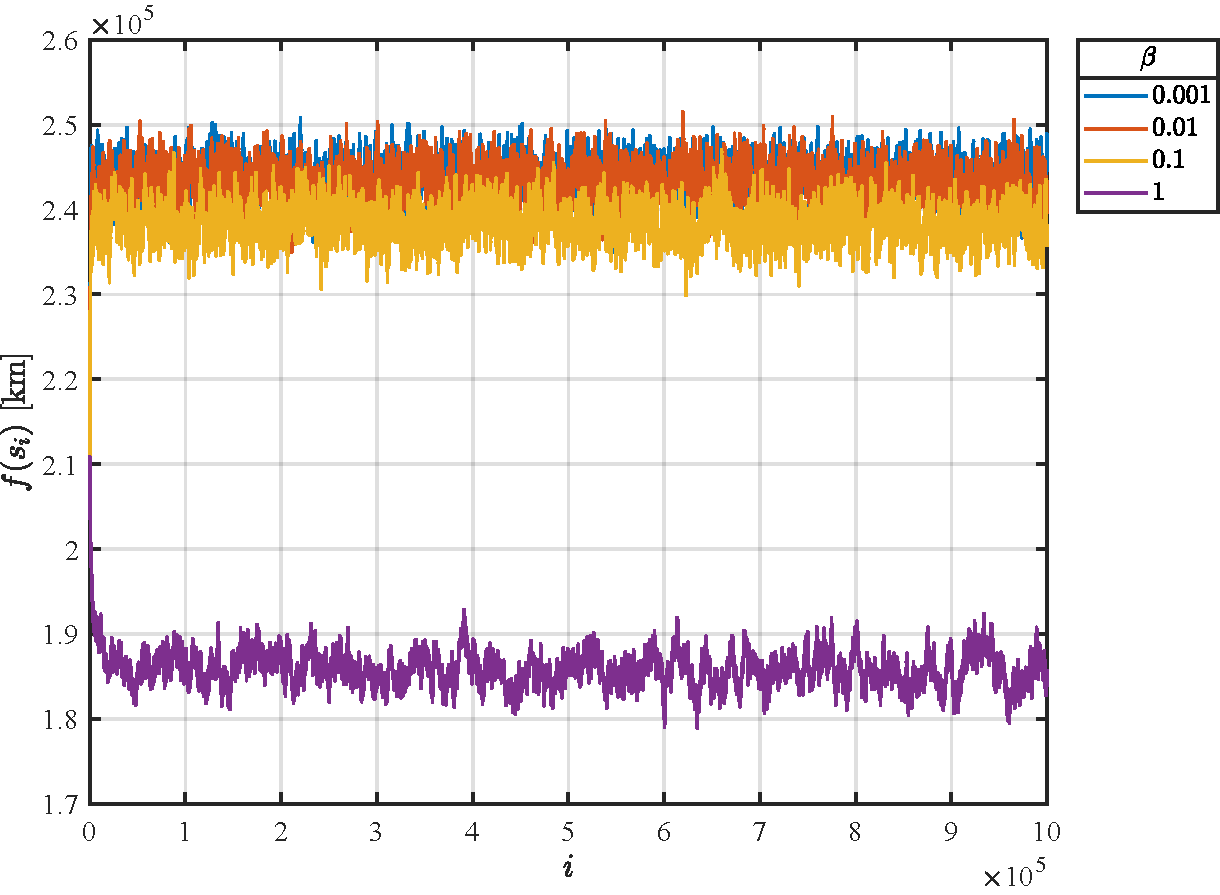
\includegraphics[width=0.9\textwidth]{resources/pdf/belgium_bad_rand.pdf}
        \noskipcaption{Évolution de la longueur du chemin au cours des itérations pour de faibles valeurs de $\beta$ et une initialisation aléatoire dans le cas de la Belgique.}
    \end{figure}
    Nous constatons que pour de faibles valeurs de $\beta$ (inférieures à 1), les longueurs obtenues oscillent et ne semblent pas converger vers une solution optimale. Si le résultat obtenu est meilleur que l'initial, c'est en réalité le fruit du hasard.
    \begin{figure}[H]
        \centering
        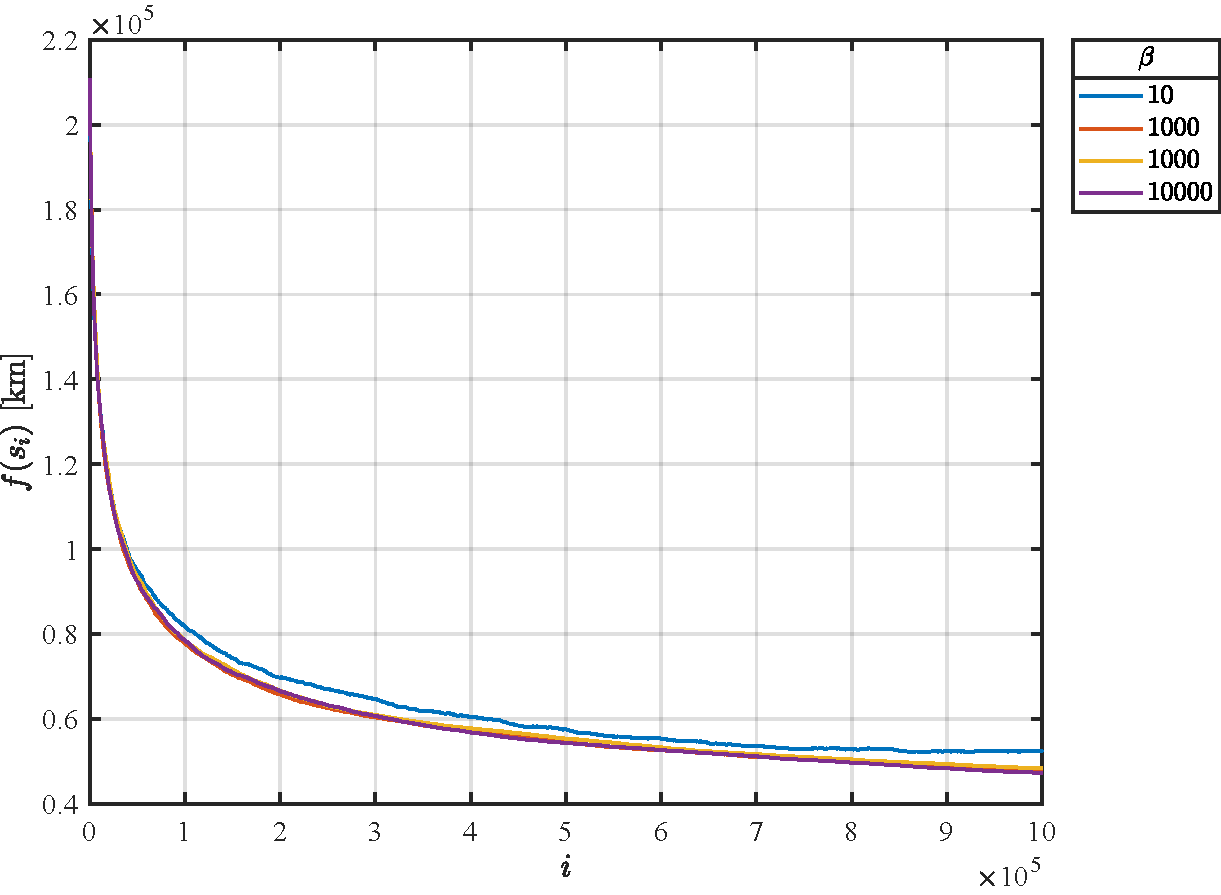
\includegraphics[width=0.9\textwidth]{resources/pdf/belgium_fine_rand.pdf}
        \noskipcaption{Évolution de la longueur du chemin au cours des itérations pour des valeurs élevées de $\beta$ et une initialisation aléatoire dans le cas de la Belgique.}
    \end{figure}
    Au contraire, puisque le chemin initial est mal choisi, une valeur élevée de $\beta$ pousse l'algorithme à \og{}descendre\fg{} presque tout le temps vers des solutions meilleures sans jamais revenir sur ses pas puisqu'il est toujours possible de trouver mieux. \par
    À condition qu'il soit bien choisi, un $\beta$ fixe permet donc une convergence intéressante, et plutôt rapide, vers une solution acceptable. Cependant, cette convergence ralentit rapidement il est donc inenvisageable de trouver la solution optimale à partir d'un mauvais chemin initial.
    \subsection{Initialisation déterministe}
    Pour cette étude, nous avons déterminé le chemin initial de chaque instance du problème avec l'algorithme déterministe du plus proche voisin (cf. section \ref{sec:NNA}). Pour rappel,
    \begin{table}[H]
    	\centering
    	\begin{tabular}{|c|c|c|}
    		\hline
    		Instance & Longueur de $s_{ini}$ $\sbk{\si{\kilo\meter}}$ & Qualité de $s_{ini}$ \\ \hline
    		\hline
    		Djibouti & \num{6770} & \num{1.0017}\\ \hline
    		Qatar & \num{11330} & \num{1.2115}\\ \hline
    		Belgique & \num{8822} & \num{1.2232}\\ \hline
    	\end{tabular}
    	\noskipcaption{Longueurs et qualités des chemins initialisés par l'algorithme du plus proche voisin.}
    	\label{tab:q5_2}
    \end{table}
    \subsubsection{Première évaluation}
    Pour cette première évaluation, nous avons procédé de la même manière que pour l'initialisation aléatoire. Les résultats sont présentés à la table \ref{tab:beta_for_heuristic}.\par
    \begin{table}[H]
    	\centering
    	\begin{tabular}{|l|c|c|c|c|c|c|c|}
    		\cline{2-8}
    		\multicolumn{1}{c|}{} & \multicolumn{7}{c|}{$\beta$} \\ \hline
    		Instance & \num{0.01} & \num{0.1} & \num{1} & \num{10} & \num{100} & \num{1000} & \num{10000}\\ \hline
    		\hline
    		Djibouti & \num{6770} & \num{6770} & \num{6770} & \num{6659} & \num{6659} & \num{6664} & \num{6664}\\ \hline
    		Qatar & \num{11330} & \num{11330} & \num{11330} & \num{10452} & \num{10838} & \num{10877} & \num{10891}\\ \hline
    		Belgique & \num{8822} & \num{8822} & \num{8822} & \num{8685} & \num{8644} & \num{8653} & \num{8666}\\ \hline
    	\end{tabular}
    	\noskipcaption{Longueurs moyennes des chemins calculés des instances du problème, pour des valeurs de $\beta$ différentes et une initialisation déterministe.}
    	\label{tab:beta_for_heuristic}
    \end{table}
    Nous constatons immédiatement que, pour les 3 instances du problème, une faible valeur de $\beta$ (à priori inférieure à 1) ne fournit pas de résultats satisfaisants\footnote{La distance minimale obtenue est identique à celle de l'initialisation, \cad{} qu'aucun chemin visité durant l'exécution de l'algorithme ne fournit de meilleure distance que le chemin initial.}. En réalité, une valeur trop petite de $\beta$ rend l'algorithme insensible à la variation de longueur et la distribution de probabilité en devient quasiment uniforme, rendant impossible toute convergence. \par
    En ce qui concerne les valeurs de $\beta$ supérieures à 1, nous observons qu'à partir d'un certain seuil ($\beta \pm 10$), augmenter la valeur de $\beta$ n'améliore plus les résultats. En effet, lorsque $\beta$ prend des valeurs excessives ($\beta = \num{1000}$, $\beta = \num{10000}$), les remplacements contre-productifs ($\Delta > 0$) génèrent des $\alpha$ trop petit
    pour qu'ils soient effectués dans un nombre d'itérations raisonnable. En quelques sortes, l'algorithme ne revient jamais sur ses pas ce qui augmente le phénomène de stagnation.
    \subsubsection{Deuxième évaluation}
    Pour cette seconde évaluation, nous avons conservé la valeur $\beta = 10$. En effet, celle-ci, au vu de l'analyse précédente, semble fournir les résultats les plus intéressants.\par
    Comme précédemment, nous allons relancer l'algorithme en augmentant progressivement le nombre d'itérations effectuées.\par
    Les qualités des solutions obtenues sont présentées à la table \ref{tab:quality_for_heuristic}.\par
    \begin{table}[H]
    	\centering
    	\begin{tabular}{|l|c|c|c|c|c|}
    		\hline
    		Nombre d'itérations & \num{e4} & \num{e5} & \num{e6} & \num{e7} & \num{e8}\\ \hline
    		\hline
    		Djibouti & \num{1} & \num{1} & \num{1} & \num{1} & \num{1}\\ \hline
    		Qatar & \num{1.1844} & \num{1.1715} & \num{1.1576} & \num{1.1433} & \num{1.1431}\\ \hline
    		Belgique & \num{1.2233} & \num{1.2215} & \num{1.2208} & \num{1.2036} & \num{1.1911}\\ \hline
    	\end{tabular}
    	\caption{Qualité des chemins calculés des instances du problème, pour $\beta = 10$ et une initialisation déterministe.}
    	\label{tab:quality_for_heuristic}
    \end{table}
    Une fois de plus, la solution optimale a été atteinte pour les villes de Djibouti, mais cette fois-ci en seulement \num{e4} itérations.
    \subsubsection{Analyse des résultats}
    Comme pour la précédente analyse, nous avons ajouté des figures présentant l'évolution de la longueur du chemin au cours des itérations réalisées afin d'appuyer nos interprétations des résultats.
    \begin{figure}[H]
        \centering
        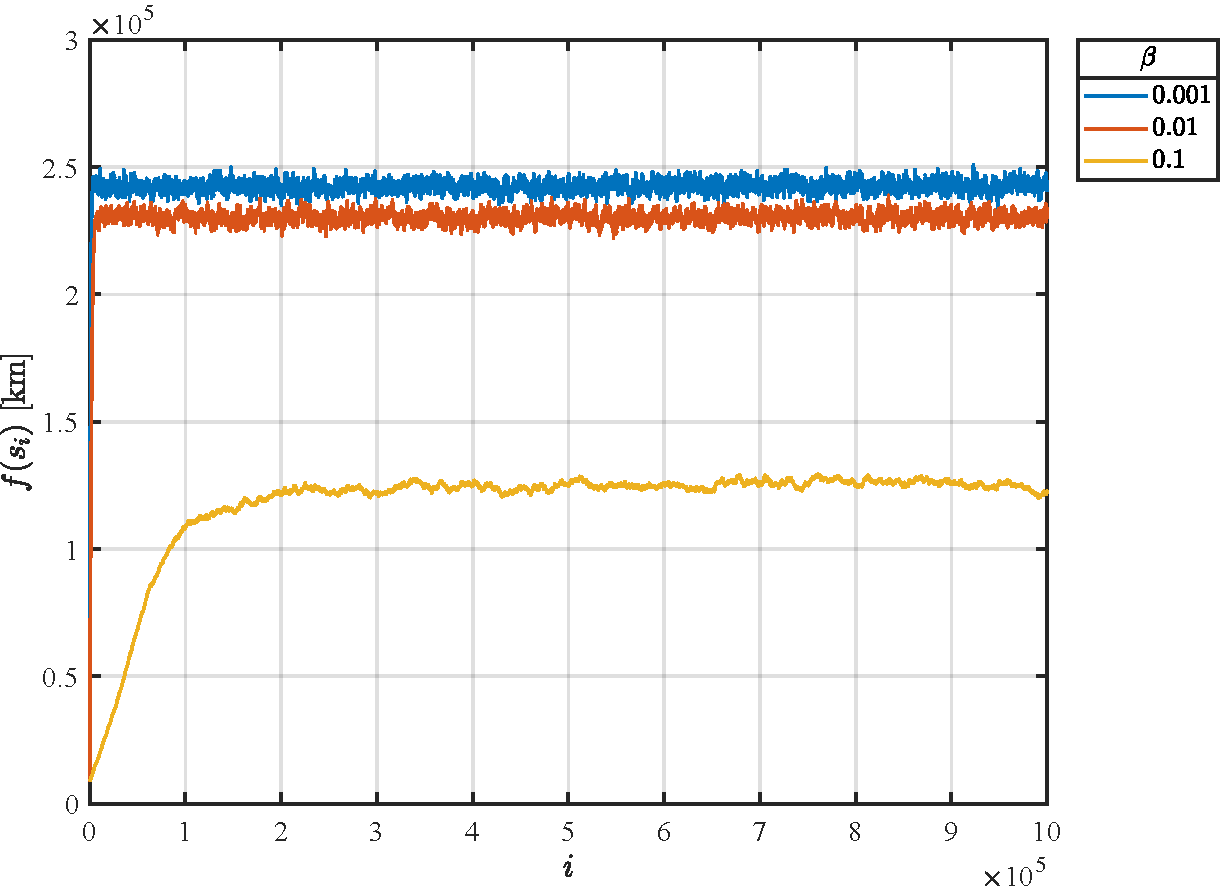
\includegraphics[width=0.9\textwidth]{resources/pdf/belgium_bad_nna.pdf}
        \noskipcaption{Évolution de la longueur du chemin au cours des itérations pour de faibles valeurs de $\beta$ et un initialisation déterministe dans le cas de la Belgique.}
    \end{figure}
    Pour des valeurs de $\beta$ (inférieures à 1), nous observons le même phénomène que pour l'initialisation aléatoire : les longueurs des chemins oscillent assez rapidement et ne convergent pas vers une solution optimale.
    \begin{figure}[H]
        \centering
        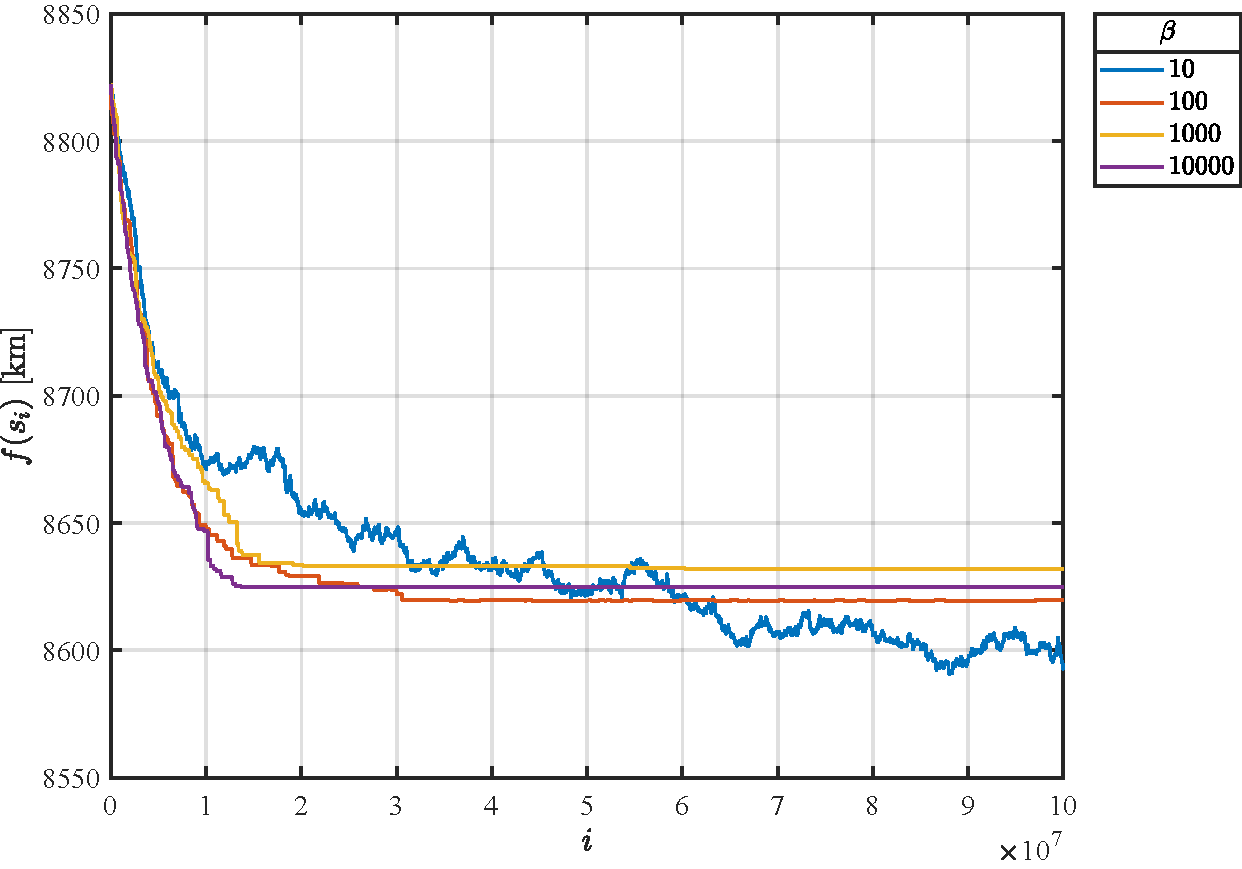
\includegraphics[width=0.9\textwidth]{resources/pdf/belgium_fine_nna.pdf}
        \noskipcaption{Évolution de la longueur du chemin au cours des itérations pour des valeurs élevées de $\beta$ et un initialisation déterministe dans le cas de la Belgique.}
    \end{figure}
    Pour des valeurs de $\beta$ excessives (typiquement supérieure à 100), on observe le phénomène décrit précédemment : l'algorithme ne revient jamais sur ses pas et stagne. Pourtant, comme dans la vraie vie, il est parfois nécessaire de prendre du recul pour repartir de plus belle. \par
    C'est pourquoi le cas $\beta = 10$ est intéressant. Il montre une convergence relativement constante vers une solution optimale tout en permettant des \og{}retours en arrière\fg{} que les valeurs supérieures n'autorisent pas.
	\section{Étude du paramètre $\beta$}
	Dans cette section, nous allons refaire une étude du paramètre $\beta$ mais cette fois en le faisant varier au cours des itérations.
	\subsection{Incrément constant}
	La première manière de modifier $\beta$ qui nous est venue à l'esprit est de l'incrémenter constamment au fil des itérations. Cependant, que ce soit de manière linéaire (\texttt{beta = beta + x}) ou exponentielle (\texttt{beta = beta * x}), nous nous sommes aperçu rapidement de l'inefficacité de la méthode. \par 
	En effet, cela a eu pour seul effet de réduire la vitesse de convergence de notre algorithme et cela pour les mêmes raisons qu'un $\beta$ constant trop élevé. \par
	En réalité, augmenter $\beta$ permet de trouver plus rapidement un minimum local, mais ce n'est pas réellement ce qui est recherché pour le problème du voyageur de commerce.
	\subsection{Recuit simulé}
	En nous renseignant sur les différentes méthodes de mise à jour de $\beta$, nous sommes tombés sur la méthode dite du \textit{recuit simulé} \cite{yang2014nature}. Inspirée de la métallurgie, elle consiste à \og{}réchauffer\fg{} une solution stagnante pour lui permettre, peut-être, d'atteindre un meilleur minimum. Dans notre cas, réchauffer la solution signifie diminuer $\beta$ brièvement et ainsi permettre un léger \og{}retour en arrière\fg{}. \par
	Dans notre implémentation de cette méthode, pour quantifier la stagnation de nos itérations, nous avons divisé la longueur courante par la longueur moyenne des chemins précédents. Si ce rapport $r$ est proche de $1$, cela signifie que l'algorithme stagne. \par 
	Ensuite, nous avons remplacé $\beta$ dans l'évaluation de $\alpha$ par une fonction de $r$, diminuant lorsque $r$ s'approche de $1$. Plusieurs fonctions nous sont venues à l'esprit : des paraboles centrées en $1$, des cosinus centrés en $1$, des logarithmes au carré, etc. \par
	Malheureusement, bien qu'ayant testé un grand nombre de paramètres pour ces fonctions, aucune n'a donné de meilleurs résultats qu'un simple $\beta$ constant. \par
	En réalité, cela n'est pas étonnant. Grâce à la distribution de probabilité que nous avons choisie, beaucoup d'états sont accessibles en permanence. Il est alors assez compliqué d'atteindre un minimum local, \cad{} un état pour lequel toutes les transitions possibles sont contre-productives ($\Delta > 0$). Dès lors, il est assez rare que notre algorithme stagne réellement. \par
	Confirmant nos impressions, nous avons pu lire dans la littérature que la méthode du recuit simulé, et les méthodes similaires, étaient plus efficaces pour des problèmes possédant plusieurs solutions, comme les grilles de Sudoku par exemple.
    \section{Solution et conclusion}
    Finalement, nous avons choisi un $\beta$ constant égal à \num{10}. Cette valeur à l'avantage de fournir des solutions acceptables pour les trois instances du problème et offre une convergence appréciable. \par
    Aussi, nous avons préféré initialiser la chaîne de Markov à l'aide de l'algorithme du plus proche voisin car l'initialisation aléatoire fournissait des résultats déplorables. \par
    Finalement, pour déterminer la meilleure solution possible\footnote{Il est bien entendu possible d'obtenir mieux en augmentant le nombre d'itérations.}, nous avons exécuté notre algorithme avec un nombre d'itérations ridiculement grand, à savoir \num{e10}. \par
    Après un temps de calcul de \SI{3325.1915}{\second}, \cad{} un peu moins d'une heure, nous avons obtenu un chemin, représenté à la Figure \ref{fig:final_solution}, d'une longueur de \SI{8473.7947}{\kilo\meter}.
    \begin{figure}[H]
        \centering
        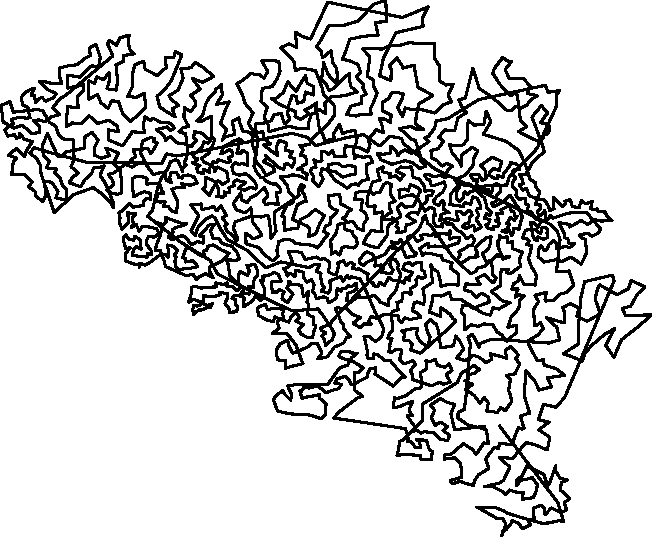
\includegraphics[width=0.8\textwidth]{resources/pdf/final.pdf}
        \noskipcaption{Solution au problème du voyageur de commerce, pour l'instance de la Belgique, en \num{e10} itérations de l'algorithme de Metropolis-Hastings.}
        \label{fig:final_solution}
    \end{figure}
    Visiblement, cette solution n'est pas la solution optimale : encore beaucoup de segments sont tracés entre deux villes éloignées. Néanmoins, on peut observer que, pour la plupart du chemin, le choix des passages n'est pas fait de manière inconsidérée. \par
    En conclusion, pour un problème \emph{NP-hard}, la solution trouvée n'est pas si mauvaise et le temps de calcul reste respectable. Cependant, il est à noter que la qualité de la solution n'a pas été améliorée de manière transcendante vis à vis de celle de l'algorithme du plus proche voisin. Il est donc important de relativiser le travail effectué par Metropolis-Hastings : n'aurait-on pas pu nous satisfaire du chemin initial ?
	\newpage
	\printbibliography
\end{document}
